\documentclass[a4paper,12pt,oneside,openany,table,xcdraw]{article}

\usepackage{setspace}
\usepackage{multirow}
\usepackage{hyperref}
\usepackage{caption}
\usepackage{indentfirst}

\usepackage[brazilian]{babel}
\usepackage[utf8x]{inputenc}
\usepackage{amsmath, graphicx, enumerate}
\usepackage{float, verbatim}
\usepackage[colorinlistoftodos]{todonotes}
\usepackage{makeidx} % Para o sumário
\usepackage{geometry}

\geometry{a4paper, hmargin={3cm, 3cm}, vmargin={3cm, 2cm} }
\setlength{\parindent}{1.0cm}

\begin{document}
\newcommand{\thedepartment}{Faculdade de Engenharia Elétrica}
\newcommand{\thecourse}{FEELT}
\newcommand{\thetitle}{CIRCUITOS TRIFÁSICOS EQUILIBRADOS}
\newcommand{\thetype}{Relatório da Disciplina de Experimental de Circuitos Elétricos II}
\newcommand{\theproftitle}{Bacharel em Engenharia Elétrica}
\newcommand{\thestudent}{Lesly Viviane Montúfar Berrios\\
\centering11811ETE001}
\newcommand{\theadvisor}{Prof. Wellington Maycon Santos Bernardes}
\newcommand{\thecity}{Uberlândia}

\thispagestyle{empty}\newcommand*{\themonth}{\ifthenelse{\the\month < 2}{Janeiro }
                  {\ifthenelse{\the\month < 3}{Fevereiro }
                  {\ifthenelse{\the\month < 4}{Março }
                  {\ifthenelse{\the\month < 5}{Abril }
                  {\ifthenelse{\the\month < 6}{Maio }
                  {\ifthenelse{\the\month < 7}{Junho }
                  {\ifthenelse{\the\month < 8}{Julho }
                  {\ifthenelse{\the\month < 9}{Agosto }
                  {\ifthenelse{\the\month < 10}{Setembro }
                  {\ifthenelse{\the\month < 11}{Outubro }
                  {\ifthenelse{\the\month < 12}{Novembro }{Dezembro }}}}}}}}}}}}
                  
\begin{titlepage}
\begin{center}

	\vspace{-0.5cm}

  \begin{figure}[hbt!]
		\begin{center}
		   
\includegraphics[width=2.8cm]{ufu-logo.png}
		\end{center}
	\end{figure}
 	%\vspace{-4cm}

%\begin{doublespacing}

  \Large{\textbf{Universidade Federal de Uberlândia}}\\
  \large{\thedepartment}\\
  \large{\thecourse}\\


\vspace{5.8cm}
  \par
  \large\textbf{\thetitle}
\vspace{5.8cm} 

%\end{doublespacing}
  \par
  \thetype\\
  por\\
  %\hspace{2cm}\large{}\\

\vspace{0.8cm}
\par
  \normalsize{\thestudent}\\ [2cm]
  \theadvisor

\par\vfill
  \thecity, \themonth / \the\year

\end{center}

\end{titlepage}

%% Comeca o documento !

\onehalfspacing
\tableofcontents % sumário
\newpage

\section{Objetivos} % 2,5%
Verificar experimentalmente os conceitos teóricos sobre as relações existentes entre tensões de fases $V_F$ e de linhas $V_L$ em cargas ligadas em estrela, e correntes de fases $I_F$ e de linhas $I_L$ em cargas ligadas em triângulo. Além disso, comparar os resultados com os valores obtidos utilizando uma análise teórica. 

\section{Introdução teórica} % 5%
As primeiras linhas de transmissão de energia elétrica, que surgiram no final do século XIX, destinavam-se exclusivamente ao suprimento do sistema de iluminação, pequenos motores e sistema de tração (railway) e operavam em corrente contínua a baixa magnitude de tensão. A geração e transmissão usando os mesmos níveis de tensão das diferentes cargas restringiu a distância entre a planta de geração e os consumidores e a tensão da geração em corrente contínua não podia ser facilmente aumentada para a transmissão a grandes distâncias \cite{ph}. 

Para realizar uma transmissão de energia elétrica a grandes distâncias era necessário um nível elevado de magnitude de tensão, e essa tecnologia de conversão para corrente contínua não era viável naquela época. Por isso, foi necessária a mudança da transmissão de corrente continua para corrente alternada, devido principalmente aos seguintes motivos:

\begin{itemize}
\item O desenvolvimento e uso dos transformadores, permitindo a transmissão a grandes distâncias usando altos níveis de tensão, reduzindo as perdas elétricas dos sistemas e a queda de tensão.
\item A elevação/redução da magnitude de tensão é realizado com uma alta eficiência e a baixo custo através dos transformadores.
\item Surgimento de geradores e motores em corrente alternada, construtivamente mais simples, eficientes e baratos que as máquinas em corrente contínua
\end{itemize}

Assim, a corrente alternada seria a melhor alternativa para a transmissão de energia elétrica à grandes distâncias. Além disso, introduz-se o conceito de gerador trifásico, ilustrado pela Figura \ref{gerador}, no qual três bobinas defasadas em 120 graus elétricos no espaço geram um conjunto de três tensões de mesmo valor máximo, defasadas de 120 graus elétricos no tempo.

Um gerador trifásico aproveita melhor o espaço físico, resultando em um gerador de tamanho reduzido e mais barato, comparado com os geradores monofásicos de igual potência, ademais são superiores aos motores monofásicos em rendimento, tamanho, fator de potência e capacidade de sobrecarga.
Um sistema monofásico precisa de dois condutores; e um sistema trifásico (perfeitamente balanceado) precisa de três condutores, porém conduz três vezes mais potência. Na prática, devido a pequenos desequilíbrios inevitáveis, os sistemas trifásicos contam com um quarto condutor, o neutro.

É possivel conectar as bobinas de gerador trifásicos em configuração estrela ou delta, assim como a carga em \emph{Conexão em estrela} (\ref{estrela}) ou  \emph{Conexão em delta/triângulo} (\ref{delta}).
\begin{figure}[H]
\centering
\captionsetup{font=scriptsize}
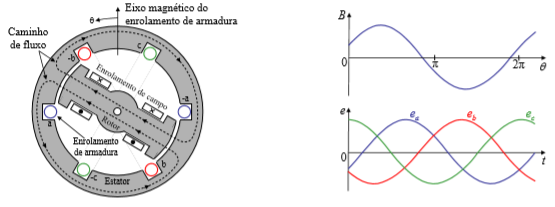
\includegraphics[width=14.5cm]{motor3phi}
\caption{Geração de tensão alternada trifásica.}
\label{gerador}
\end{figure}

\subsection{Carga em conexão em estrela} \label{estrela}
A carga na configuração estrela é caracterizada por ter uma tensão fase-neutro entre seus terminais e corrente de linha igual à corrente de fase ($I_L=I_F$). Ainda é possível determinar a tensão fase-fase ou de linha pela relação descrita na Figura \ref{carga-estrela} \cite{irwin}. 
\begin{figure}[H]
\centering
\captionsetup{font=scriptsize}
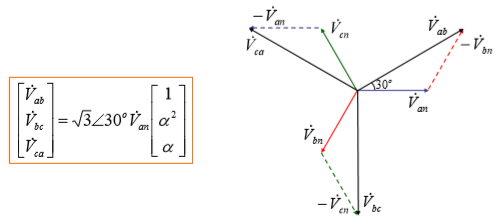
\includegraphics[width=14.5cm]{carga-estrela}
\caption{Relação entre tensão de linha e fase numa carga em estrela.}
\label{carga-estrela}
\end{figure}

\subsection{Carga em conexão em delta ou triângulo} \label{delta}
Já para a carga na configuração delta, ou triângulo, em seus terminais há uma tensão de linha igual a tensão de fase \cite{irwin}. Nesse caso, a relação entre linha e fase ocorre para a corrente, conforme descrito na Figura \ref{carga-delta}.
\begin{figure}[H]
\centering
\captionsetup{font=scriptsize}
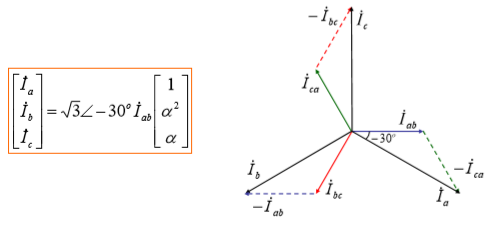
\includegraphics[width=14.5cm]{carga-delta}
\caption{Relação entre corrente de linha e fase numa carga em delta.}
\label{carga-delta}
\end{figure}

\section{Preparação}
\subsection{Materiais e ferramentas} % 2,5%
\begin{enumerate}[1 -]
\item \emph{\textbf{Fonte:}}
Alimentará todo o circuito. Possui frequência de $60Hz$.

\item \emph{\textbf{Regulador de tensão (Varivolt):}}
Também chamado de autotransformador, permitirá obter o valor desejado de corrente a partir da regulagem correta da tensão fornecida pela fonte.

\item \emph{\textbf{Conectores:}}
Para as conexões no circuito foi utilizado majoritariamente cabos banana-banana.

\item \emph{\textbf{Medidor eletrônico KRON Mult K:}}
Possibilita encontrar a medição da potência real (P) - vatímetro, reativa (Q) e aparente (S) do circuito. Ele também possui função de cofasímetro, instrumento elétrico que mede o fator de potência (fp, $cos\theta$) ou o ângulo da impedância $\theta$ do circuito, para um circuito com a impedância $Z = Z\angle \theta$.

\item \emph{\textbf{Amperímetro analógico AC:}}
Instrumento utilizado para acompanhar visualmente o aumento da corrente.

\item \emph{\textbf{Reatores de 160 mH:}}
Foram utilizados 3, para compor a carga do circuito trifásico. Sendo $L=160mH$ e $R_L=3,8\Omega$.

\item \emph{\textbf{Resistores de $50\Omega$:}}
Foram utilizados 3, para compor a carga do circuito trifásico.
\end{enumerate}

\subsection{Montagem} % 2,5%

\subsubsection{Carga em estrela}
Observe a montagem indicada na Figura \ref{fig1} abaixo, alimentando os pontos a b c n através de uma fonte alternada trifásica em seqüência de fases abc (ou direta), aplicando uma tensão entre linhas $V_L$ igual a 100 V, em frequência de 60 Hz.

Os parâmetros da carga são: $R = 50\Omega$; $R_L = 3,8 \Omega$; $L = 160 mH$. Na Figura \ref{fig1}, $V_L$ representa um voltímetro conectado para medir a tensão entre linhas (fases ab); $V_F$ representa um voltímetro conectado para medir a tensão de fase (fases cn, por exemplo); $A_L$ representa um amperímetro conectado para medir a corrente de linha (igual a de fase) e; $A_N$ representa um amperímetro conectado para medir a corrente no fio neutro. 
\begin{figure}[H]
\centering
\captionsetup{font=scriptsize}
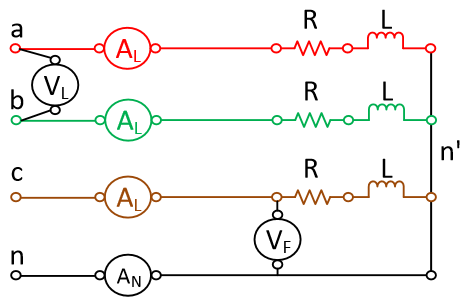
\includegraphics[width=14cm]{fig1}
\caption{Ligação em estrela em sequência de fases abc ($n = n’$).}
\label{fig1}
\end{figure}
Observa-se pelo desenho que não é possível obter a tensão e corrente de todas as fases de forma simultânea, sendo necessária a mudança dos medidores $V_L$ e $V_F$ para a obtenção dos demais valores. Para isso, utilizaremos o medidor trifásico eletrônico \textit{Kron Mult-K} (wattímetro),  usando as entradas $V_A$, $V_B$, $V_C$, $V_N$ para as medidas de tensão e $I_A$, $I_B$ e $I_C$ para as medidas de corrente, assim sendo, realizando as ligações apropriadas. Como o \textit{Kron} não mede a corrente de neutro, então é necessário um amperímetro analógico AC entre $n$ e $n’$.

\begin{figure}[H]
\centering
\captionsetup{font=scriptsize}
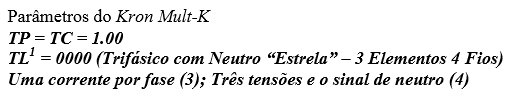
\includegraphics[width=13.5cm]{parametros1}
\end{figure}

Com o \textit{Kron Mult-K} configurado com os parâmetros acima, foi possível obter as grandezas das Tabelas \ref{tab1} e \ref{tab2}, sendo a primeira com neutro conectado e a segunda sem neutro conectado.

\begin{table}[H]\scriptsize
\centering
\def\arraystretch{1.35}
\captionsetup{font=scriptsize}
\captionof{table}{Conexão em estrela com neutro conectado.} \label{tab1}

\begin{tabular}{|c|c|c|c|c|c|c|c|c|c|}
\hline
$V_{L} (V)$ & $V_{F} (V)$ & $I_{L} (A)$ & $I_{N} (A)$        & $P_{F} (W)$ & $P_{T} (W)$       & $Q_{F} (Var)$ & $Q_{T} (Var)$     & $S_{F} (VA)$ & $S_{T} (VA)$      \\ \hline
100,3       & 59,6           & 0,636       & \multirow{3}{*}{0} & 22,42       & \multirow{3}{*}{67,26} & 28,4          & \multirow{3}{*}{85,2} &  36,18            & \multirow{3}{*}{108,5} \\ \cline{1-3} \cline{5-5} \cline{7-7} \cline{9-9}
100,3       & 59,6           &  0,636           &                    & 22,42       &                   & 28,4              &                   &   36,18            &                   \\ \cline{1-3} \cline{5-5} \cline{7-7} \cline{9-9}
100,3       & 59,6           &   0,636          &                    & 22,42       &                   &  28,4             &                   & 36,18              &                   \\ \hline
\end{tabular}
\end{table}

\begin{table}[H]\scriptsize
\centering
\def\arraystretch{1.35}
\captionsetup{font=scriptsize}
\captionof{table}{Conexão em estrela sem neutro conectado.} \label{tab2}

\begin{tabular}{|c|c|c|c|c|c|c|c|c|c|}
\hline
$V_{L} (V)$ & $V_{F} (V)$  & $I_{L} (A)$ & $I_{N} (A)$        & $P_{F} (W)$ & $P_{T} (W)$       & $Q_{F} (Var)$ & $Q_{T} (Var)$     & $S_{F} (VA)$ & $S_{T} (VA)$      \\ \hline
100,4       & 57,9           & 0,627       & \multirow{3}{*}{-} & 22,64       & \multirow{3}{*}{67,92} & 28,29         & \multirow{3}{*}{84,87} &  36,23            & \multirow{3}{*}{108,7} \\ \cline{1-3} \cline{5-5} \cline{7-7} \cline{9-9}
100,4       & 57,9           & 0,627              &                    & 22,64       &                   &  28,29             &                   &   36,23                      &                   \\ \cline{1-3} \cline{5-5} \cline{7-7} \cline{9-9}
100,4       & 57,9           &  0,627             &                    & 22,64       &                   &  28,29             &                   &  36,23                       &                   \\ \hline
\end{tabular}
\end{table}

Agora, conecte somente $I_A$, $V_A$ e $V_N$ do medidor eletrônico \emph{Kron Mult-K}, e encontre os valores da Tabela \ref{tab3} e \ref{tab4} com a seguinte configuração: 
\begin{figure}[H]
\centering
\captionsetup{font=scriptsize}
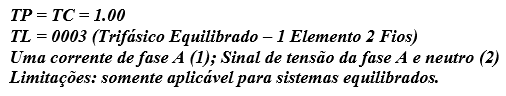
\includegraphics[width=13.5cm]{parametros2}
\end{figure}


\begin{table}[H]\scriptsize
\centering
\def\arraystretch{1.35}
\captionsetup{font=scriptsize}
\captionof{table}{Conexão em estrela com neutro conectado (0003 - sistema equilibrado).} \label{tab3}

\begin{tabular}{|c|c|c|c|c|c|c|c|c|c|}
\hline
$V_{L} (V)$ & $V_{F} (V)$ & $I_{L} (A)$ & $I_{N} (A)$        & $P_{F} (W)$ & $P_{T} (W)$             & $Q_{F} (Var)$ & $Q_{T} (Var)$           & $S_{F} (VA)$ & $S_{T} (VA)$           \\ \hline
100,4       & 57,96          & 0,636       & \multirow{3}{*}{0} & 67,38       & \multirow{3}{*}{202,14} & 87,46         & \multirow{3}{*}{262,38} & 110,7        & \multirow{3}{*}{332,1} \\ \cline{1-3} \cline{5-5} \cline{7-7} \cline{9-9}
100,4       & 57,96          & 0,636       &                    & 67,38       &                         & 87,46         &                         & 110,7        &                        \\ \cline{1-3} \cline{5-5} \cline{7-7} \cline{9-9}
100,4       & 57,96          & 0,636       &                    & 67,38       &                         & 87,46         &                         & 110,7        &                        \\ \hline
\end{tabular}
\end{table}

\begin{table}[H]\scriptsize
\centering
\def\arraystretch{1.35}
\captionsetup{font=scriptsize}
\captionof{table}{Conexão em estrela sem neutro conectado (0003 - sistema equilibrado).} \label{tab4}

\begin{tabular}{|c|c|c|c|c|c|c|c|c|c|}
\hline
$V_{L} (V)$ & $V_{F} (V)$ & $I_{L} (A)$ & $I_{N} (A)$        & $P_{F} (W)$ & $P_{T} (W)$             & $Q_{F} (Var)$ & $Q_{T} (Var)$           & $S_{F} (VA)$ & $S_{T} (VA)$           \\ \hline
100,0       & 57,74          & 0,634       & \multirow{3}{*}{-} & 66,89       & \multirow{3}{*}{200,67} & 87,03         & \multirow{3}{*}{261,90} & 109,6        & \multirow{3}{*}{328,8} \\ \cline{1-3} \cline{5-5} \cline{7-7} \cline{9-9}
100,0       & 57,74          & 0,634       &                    & 66,89       &                         & 87,03         &                         & 109,6        &                        \\ \cline{1-3} \cline{5-5} \cline{7-7} \cline{9-9}
100,0       & 57,74          & 0,634       &                    & 66,89       &                         & 87,03         &                         & 109,6        &                        \\ \hline
\end{tabular}
\end{table}

\subsubsection{Carga em delta}
Agora observe a montagem indicada na Figura \ref{fig2} abaixo, com a mesma
impedância anterior, só que agora com a carga conectada em triângulo. Na Figura \ref{fig2}, $V_L$
representa um voltímetro conectado para medir a tensão entre linhas; $A_F$ representa um
amperímetro conectado para medir a corrente de fase; $A_L$ representa um amperímetro
conectado para medir a corrente de linha.

Observa-se também, como no caso anterior, é necessária a mudança dos
medidores $V_L$ para a obtenção dos demais valores de tensão de linha. Para isso,
utilizaremos o medidor trifásico eletrônico \emph{Kron Mult-K}, sendo as entradas $V_A$, $V_B$ e $V_C$
para as medidas de tensão e $I_A$, $I_B$ e $I_C$ para as medidas de corrente, realizando as
ligações apropriadas. A corrente $A_F$ será obtida usando o amperímetro analógico.
\begin{figure}[H]
\centering
\captionsetup{font=scriptsize}
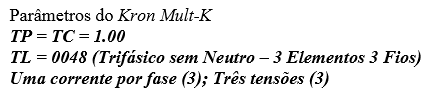
\includegraphics[width=13.5cm]{parametros3}
\end{figure}
\begin{figure}[H]
\centering
\captionsetup{font=scriptsize}
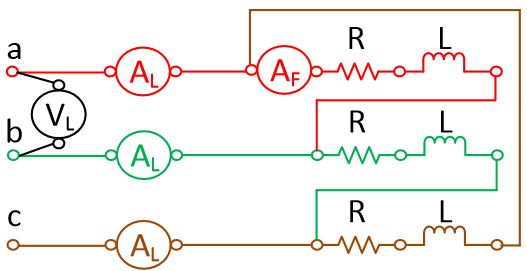
\includegraphics[width=14cm]{fig2}
\caption{Ligação em triângulo em sequência de fases abc (convencional).}
\label{fig2}
\end{figure}

Os valores dos instrumentos devem ser anotados na Tabela \ref{tab5}.

\begin{table}[H]\scriptsize
\centering
\def\arraystretch{1.35}
\captionsetup{font=scriptsize}
\captionof{table}{Conexão em delta ($TL=0048$ - Trifásico sem neutro).} \label{tab5}

\begin{tabular}{|c|c|c|c|c|c|c|c|c|c|}
\hline
$V_{L} (V)$ & $I_{F} (A)$           & $I_{L} (A)$ & $P_{F} (W)$ & $P_{T} (W)$             & $Q_{F} (Var)$ & $Q_{T} (Var)$           & $S_{F} (VA)$ & $S_{T} (VA)$            & Fator de potência \\ \hline
100,20      & \multirow{3}{*}{1,10} & 1,897       & 67,70       & \multirow{3}{*}{201,20} & 85,75         & \multirow{3}{*}{256,80} & 109,20       & \multirow{3}{*}{326,40} & 0,619             \\ \cline{1-1} \cline{3-4} \cline{6-6} \cline{8-8} \cline{10-10} 
100,00       &                       & 1,889       & 66,44       &                         & 86,20         &                         & 108,90       &                         & 0,610             \\ \cline{1-1} \cline{3-4} \cline{6-6} \cline{8-8} \cline{10-10} 
100,30      &                       & 1,879       & 67,10       &                         & 84,80         &                         & 108,30       &                         & 0,621             \\ \hline
\end{tabular}
\end{table}

Agora, conecte somente $I_A$, $I_C$, $V_A$, $V_B$ e $V_C$ (desconecte $I_B$) do medidor
eletrônico \emph{Kron Mult-K}, e encontre os valores da Tabela \ref{tab6} com a seguinte
configuração:
\begin{figure}[H]
\centering
\captionsetup{font=scriptsize}
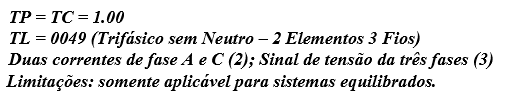
\includegraphics[width=13.5cm]{parametros4}
\end{figure}

\begin{table}[H]\scriptsize
\centering
\def\arraystretch{1.35}
\captionsetup{font=scriptsize}
\captionof{table}{Conexão em delta ($TL=0049$ - Trifásico sem neutro - equilibrado).} \label{tab6}

\begin{tabular}{|c|c|c|c|c|c|c|c|c|c|}
\hline
$V_{L} (V)$ & $I_{F} (A)$           & $I_{L} (A)$ & $P_{F} (W)$ & $P_{T} (W)$             & $Q_{F} (Var)$ & $Q_{T} (Var)$           & $S_{F} (VA)$ & $S_{T} (VA)$            & Fator de potência \\ \hline
100,20      & \multirow{3}{*}{1,10} & 1,895       & 67,65       & \multirow{3}{*}{201,00} & 85,76         & \multirow{3}{*}{256,80} & 109,20       & \multirow{3}{*}{326,10} & 0,617             \\ \cline{1-1} \cline{3-4} \cline{6-6} \cline{8-8} \cline{10-10} 
99,85       &                       & 1,885       & 66,22       &                         & 86,14         &                         & 108,70       &                         & 0,609             \\ \cline{1-1} \cline{3-4} \cline{6-6} \cline{8-8} \cline{10-10} 
100,00      &                       & 1,873       & 67,09       &                         & 84,88         &                         & 108,20       &                         & 0,622             \\ \hline
\end{tabular}
\end{table}

\section{Análise sobre segurança} % 2,5%
Os óculos de segurança são Equipamentos de Proteção Individual (EPIs) e são utilizados para a proteção da área ao redor dos olhos contra qualquer tipo de detrito estranho, que possa causar irritação ou ferimentos. Também protegem contra faíscas, respingos de produtos químicos, detritos, poeira, radiação e etc \cite{safe}.
É importante a utilização desse equipamento durante os experimentos a fim de evitar qualquer dano, além de preparar o profissional para o manejo correto e seguro de qualquer equipamento.
Além disso, foi de extrema importância a presença do professor ou técnico na verificação da montagem do circuito antes de energizá-lo. Assim, reduziu-se riscos de curtos-circuitos ou sobrecarga na rede.

\section{Cálculos, análise dos resultados e questões} % (quando houver) (70%)
\begin{enumerate}[1)]
\item Verifique a relação entre as tensões de fase (VF)  e de linha (VL) obtidas a partir da montagem da Figura \ref{fig1}\\
\textbf{Resposta.} Da primeira montagem tem-se $V_L=100,3$ e $V_F=59,06$, do que se confirma a relação $V_L=V_F\cdot\sqrt{3}$ da Figura \ref{carga-estrela}.

\item Para o sistema equilibrado da Figura \ref{fig1}, a soma das correntes no ponto “n” deveria ser igual ou muito próximo a zero para as tensões senoidais aplicadas. Isto aconteceu? Explique. \\
\textbf{Resposta.} Na primeira montagem, o amperímetro analógico constatou-se que a corrente que vai para o neutro $A_N\sim 0$. Confirma-se que a soma dos fasores de corrente deverá ser 0, uma vez que estão desafados igualmente de $120^\circ$.

\item Se as correntes de linhas senoidais forem somadas fasorialmente, a soma será
igual a corrente no neutro? Por quê? \\
\textbf{Resposta.} Será igual a do neutro, devido a Lei de Kirchhoff para os nós, a soma das correntes que saem do nó deve ser igual às que saem.

\item Quando o fio neutro foi interrompido, o que aconteceu com cada instrumento de
medida? As medidas foram as mesmas do caso anterior? \\
\textbf{Resposta.} Foi necessário retirar o amperímetro análogico, que media a corrente no neutro, e as medidas obtidas para esse caso foram as mesmas do caso anterior, sendo afetadas somente por incertezas instrumentais. Essa similaridade ocorre, uma vez que idealmente a tensão é zero no neutro, e no caso de circuitos equilibrados a corrente também zera, assim é como se o circuito estivesse aberto, resultando em medidas idênticas.

\item Se, desconectando-se o fio neutro, um voltímetro fosse ligado entre os pontos $n’$ e
$n$, que valor de tensão marcaria?\\
\textbf{Resposta.} Marcaria zero, já que no neutro a tensão é zero, em ambos. Logo, a diferença de potencial marcaria 0 também.

 \item A relação de tensão $V_L = \sqrt{3} V_F$ foi comprovada experimentalmente? Por quê?\\
\textbf{Resposta.} Com o neutro conectado foi possível comprovar a relação mencionada, pois o medidor \emph{Kron} tinha referencial neutro do circuito para calcular a tensão de fase, e o erro experimental é mínimo, conforme a Tabela \ref{Erros:tensao}.
 \begin{table}[H]\scriptsize
\centering
\def\arraystretch{1.35}
\captionsetup{font=scriptsize}
\captionof{table}{Erro da tensão de fase experimental, com relação à teórica.} \label{Erros:tensao}

\begin{tabular}{|c|c|c|c|}
\hline
\multicolumn{2}{|c|}{Dados experimentais} & Dados teóricos & \multirow{2}{*}{Erro (\%)} \\ \cline{1-3}
$V_{L} (V)$         & $V_{F} (V)$         & $V_{F} (A)$    &                            \\ \hline
100,30              & 57,6                & 57,91          & -0,535                      \\ \hline
100,30              & 57,6                & 57,91          & -0,535                      \\ \hline
100,30              & 57,6                & 57,91          & -0,535                      \\ \hline
\end{tabular}
\end{table}

 \item Verifique a relação entre as correntes de fase ($I_F$) e de linha ($I_L$) obtidas a partir da
montagem da Figura \ref{fig2}. Foi igual a $I_L = \sqrt{3} I_F$?\\
\textbf{Resposta.} Comparando-se o resultado experimental com o teórico percebe-se que o erro é mínimo, conforme a Tabela \ref{Erros:corrente}.
 \begin{table}[H]\scriptsize
\centering
\def\arraystretch{1.35}
\captionsetup{font=scriptsize}
\captionof{table}{Erro da corrente de fase experimental, com relação à teórica.} \label{Erros:corrente}

\begin{tabular}{|c|c|c|c|}
\hline
\multicolumn{2}{|c|}{Dados experimentais} & Dados teóricos & \multirow{2}{*}{Erro (\%)} \\ \cline{1-3}
$I_{L} (V)$    & $I_{F} (V)$              & $I_{F} (A)$    &                            \\ \hline
1,897          & \multirow{3}{*}{1,10}    & 1,095          & 0,435                      \\ \cline{1-1} \cline{3-4} 
1,889          &                          & 1,091          & 0,860                      \\ \cline{1-1} \cline{3-4} 
1,879          &                          & 1,085          & 1,397                      \\ \hline
\end{tabular}
\end{table}

 \item Observando as potências, real e reativa, trifásicas para a mesma impedância, na
conexão em estrela e na conexão em triângulo o que pode concluir?\\
\textbf{Resposta.} Pode-se concluir que as cargas, conectadas em delta ou estrela possuem mesma potência quando se analisa um cirucito equilibrado. O resulado deve-de ao fato de em ambas configurações a multiplicação $V_L\cdot I_L$ ser diretamente proporcional a um fator de $\sqrt{3}$.

 \item Explique os motivos da pequena diferença apresentada entre as tensões de linha e
de fase, mesmo sabendo que essas tensões são iguais entre si em circuitos elétricos
equilibrados, alterando-se apenas o ângulo. Neste caso, a corrente no neutro é
exatamente zero?\\
\textbf{Resposta.} No experimento constata-se que a corrente no neutro não é zero, mas próxima, o que provoca as pequenas variações nas medições de grandezas em fases distintas, porém num sistema equilibrado. Outro possível motivo pode-ser qualquer pequena reistência oriunda dos conectores, o que provoca leve desequilíbrio no sistema. 

 \item Quando $TL = 0003$, explique por que basta a corrente da fase A e a tensão $V_AN$
para que o medidor \emph{Kron} encontre as demais medidas corretamente? Aponte uma
vantagem técnica ao utilizar esse artifício.\\
\textbf{Resposta.} Na configuração $TL = 0003$, o medidor entende que o sistema do qual será retirada as informações, de tensão, corrente, potências e fator de potência, é um sistema trifásico equilibrado. Assim, é levado em consideração as características de um sistema estrela equilibrado, o qual possui corrente e tensão de linha idênticos para cada fase, podendo o circuito ser equivalente substituido por 3 circuitos monofásicos idênticos.

 \item Ainda para $TL = 0003$, qual é a tensão informada pelo medidor: de fase ou de
linha? Qual cuidado se deve ter em relação a esse experimento?\\
\textbf{Resposta.} A tensão informada é a de linha. Deve-se atentar que a configuração $TL = 0003$ é válida somente para sistemas equilibrados e não pode ser utilizada em outros experimentos nos quais não existe equilíbrio entre as cargas.

 \item Ao aumentar gradativamente a tensão do varivolt, é importante checar se os
amperímetros não se alterem bruscamente devido a um provável curto-circuito. Um
aluno observa $A_N$ no primeiro experimento. Está incorreto? Por quê?\\
\textbf{Resposta.} Está incorreto, já que deve-se checar o amperímetro conectado à linha do sistema trifásico a fim de detecção de um possível curto-circuito. Esse aluno corre o risco do sistema entrar em curto-circuito ao observar $A_N$, pois a corrente por ele mostrada, pela LKC, tende sempre a ser 0 para sistemas equilibrados e informa dado relevante sobre uma possível corrente de curto.

 \item Um aluno ao montar o primeiro experimento, à medida que altera o valor de
tensão no varivolt, verifica que a corrente $I_N$ está crescendo também. Está correto?
Comente as principais causas.\\
\textbf{Resposta.} Não está correto, uma vez no neutro para um equilibrado não deve haver circulação de corrente, devido à Lei de Kirchhoff para as Correntes (LKC). As principais causas para a existência de corrente no neutro são: circuito em desequilíbrio, ou seja, as cargas possuem distintos valores de impedância e a LKC indica que haverá corrente no neutro; mal contato numa das fases ou rompimento dos conectores, nesse caso aparece corrente no neutro que será a soma fasorial das correntes nas fases que restaram, logo de módulo $I_F$, pois estão defasadas de $120^\circ$.  

\end{enumerate}

\newpage
\section{Simulação computacional} % (10%);
\subsection{Carga em conexão estrela}
\begin{figure}[H]
\centering
\captionsetup{font=scriptsize}
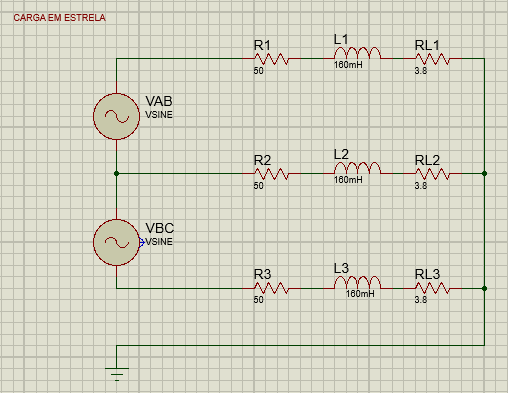
\includegraphics[width=14cm]{sim1}
\caption{Circuito da carga em conexão estrela.}
\label{sim1}
\end{figure}

\subsection{Carga em conexão delta}
\begin{figure}[H]
\centering
\captionsetup{font=scriptsize}
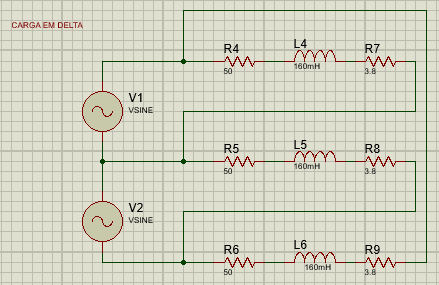
\includegraphics[width=14cm]{sim2}
\caption{Circuito da carga em conexão delta.}
\label{sim2}
\end{figure}

\section{Conclusões} % (no mínimo 10 linhas) (5%);
Neste experimento investiga-se as acerca de circuitos trifásicos equilibrados e suas particularidades em configuração delta e estrela. A análise experimental permitiu confirmar relações teóricas como $V_L=V_F\cdot\sqrt{3}$ para uma carga em estrela e $I_L = \sqrt{3}\cdot I_F$ para uma carga em delta. Além de verificar que para ambas configurações as potências (real e reativa) são as mesmas, devido as às duas relações teóricas já mencionadas apresentarem certa simetria.

Outro ponto importante verificado neste experimento é a inexistência de corrente no neutro para um circuito equilibrado. Assim, não é correto conferir corrente de curto-circuito pela corrente no neutro, já que idelamente tem valor nulo. As principais causas para a existência de corrente no neutro são: circuito em desequilíbrio, ou seja, as cargas possuem distintos valores de impedância e a LKC indica que haverá corrente no neutro; mal contato numa das fases ou rompimento dos conectores, nesse caso aparece corrente no neutro que será a soma fasorial das correntes nas fases que restaram, logo de módulo $I_F$, pois estão defasadas de $120^\circ$.  

\newpage
\begin{thebibliography}{9} 
% Introdução
\bibitem{ph}
    P. H. O. Rezende,
    "Circuitos Polifásicos Equilibrados", 2018.

\bibitem{irwin}
    J. D. Irwin,
    “Análise de Circuitos Em Engenharia”, Pearson, $4^a$ Ed., 2000.

\bibitem{boylestad}
    R. L. Boylestad,
    “Introdução À Análise de Circuitos”, Pearson, $10^a$ Ed., 2004.

\bibitem{safe}
    SafetyTrabi,
    “Óculos de segurança: Saiba quando utilizar este EPI”, SafetyTrab, 2019.
 Disponível em:
 \url{https://www.safetytrab.com.br/blog/oculos-de-seguranca/}. Acesso em: ago. 2019.


\end{thebibliography}
\end{document}
